\documentclass[rnaas]{aastex62}

\pdfoutput=1

\usepackage{lmodern}
\usepackage{microtype}
\usepackage{url}
\usepackage{amsmath}
\usepackage{amssymb}
\usepackage{natbib}
\usepackage{multirow}
\usepackage{graphicx}
\bibliographystyle{aasjournal}

% ------------------ %
% end of AASTeX mods %
% ------------------ %

% Projects:
\newcommand{\project}[1]{\textsf{#1}}
\newcommand{\kepler}{\project{Kepler}}
\newcommand{\ktwo}{\project{K2}}

% references to text content
\newcommand{\documentname}{\textsl{Note}}
\newcommand{\figureref}[1]{\ref{fig:#1}}
\newcommand{\Figure}[1]{Figure~\figureref{#1}}
\newcommand{\figurelabel}[1]{\label{fig:#1}}
\renewcommand{\eqref}[1]{\ref{eq:#1}}
\newcommand{\Eq}[1]{Equation~(\eqref{#1})}
\newcommand{\eq}[1]{\Eq{#1}}
\newcommand{\eqalt}[1]{Equation~\eqref{#1}}
\newcommand{\eqlabel}[1]{\label{eq:#1}}

% TODOs
\newcommand{\todo}[3]{{\color{#2}\emph{#1}: #3}}
\newcommand{\dfmtodo}[1]{\todo{DFM}{red}{#1}}
\newcommand{\alltodo}[1]{\todo{TEAM}{red}{#1}}
\newcommand{\citeme}{{\color{red}(citation needed)}}

% math
\newcommand{\T}{\ensuremath{\mathrm{T}}}
\newcommand{\dd}{\ensuremath{ \mathrm{d}}}
\newcommand{\unit}[1]{{\ensuremath{ \mathrm{#1}}}}
\newcommand{\bvec}[1]{{\ensuremath{\boldsymbol{#1}}}}
\newcommand{\Gaussian}[3]{\ensuremath{\frac{1}{|2\pi #2|^\frac{1}{2}}
            \exp\left[ -\frac{1}{2}#1^\top #2^{-1} #1 \right]}}

% VECTORS AND MATRICES USED IN THIS PAPER
\newcommand{\Normal}{\ensuremath{\mathcal{N}}}
\newcommand{\mA}{\ensuremath{\bvec{A}}}
\newcommand{\mC}{\ensuremath{\bvec{C}}}
\newcommand{\mS}{\ensuremath{\bvec{\Sigma}}}
\newcommand{\mL}{\ensuremath{\bvec{\Lambda}}}
\newcommand{\vw}{\ensuremath{\bvec{w}}}
\newcommand{\vy}{\ensuremath{\bvec{y}}}
\newcommand{\vt}{\ensuremath{\bvec{\theta}}}
\newcommand{\vm}{\ensuremath{\bvec{\mu}(\bvec{\theta})}}
\newcommand{\vre}{\ensuremath{\bvec{r}}}
\newcommand{\vh}{\ensuremath{\bvec{h}}}
\newcommand{\vk}{\ensuremath{\bvec{k}}}

% typography obsessions
\setlength{\parindent}{3.0ex}

\begin{document}\raggedbottom\sloppy\sloppypar\frenchspacing

\title{%
    Scalable gradients of Gaussian Process models with celerite
}

\author[0000-0002-9328-5652]{Daniel Foreman-Mackey}
\affil{Center for Computational Astrophysics, Flatiron Institute, New York, NY}

\keywords{%
methods: data analysis ---
methods: statistical
}

\section{Abstract}

This research note presents a derivation and implementation of reverse-mode
gradients of the \emph{celerite} algorithm for scalable inference with
Gaussian Process (GP) models.
These gradients can be integrated into existing automatic differentiation
frameworks to provide a scalable and computationally efficient method for
evaluating the gradients of the GP likelihood with respect to the kernel
hyperparameters.
The algorithm derived in this note uses less memory and is more efficient than
versions using automatic differentiation and the computational cost scales
linearly with the number of data points.

\section{Introduction}

Gaussian Processes \citep[GPs][]{Rasmussen:2006} are a class of models used
extensively in the astrophysical literature to model stochastic processes.
The applications are broad-ranging and some example include the time domain
variability of astronomical sources \citep{Brewer:2009, Kelly:2014,
Haywood:2014, Rajpaul:2015, Foreman-Mackey:2017}, data-driven models of light
curves or stellar spectra \citep{Wang:2012, Luger:2016, Czekala:2017}, and the
cosmic microwave background \citep{Bond:1987,Wandelt:2003}.
In all of these applications, the calculation and optimization of the GP
marginalized likelihood function (here we follow the notation of
\citealt{Foreman-Mackey:2017})
\begin{eqnarray}\eqlabel{loglike}
\log \mathcal{L}(\bvec{\theta},\,\bvec{\alpha}) &=&
    -\frac{1}{2}\,\left[\bvec{y} - \bvec{\mu}_\bvec{\theta}\right]^\T\,
        {K_\bvec{\alpha}}^{-1}\,\left[\bvec{y}-\bvec{\mu}_\bvec{\theta}\right]
    -\frac{1}{2}\,\log\det K_\bvec{\alpha} + \mathrm{constant}
\end{eqnarray}
is of central importance and this can often be the computational bottleneck.
The details of this model are omitted here (more details can be found in
\citealt{Rasmussen:2006} and \citealt{Foreman-Mackey:2017}), but the key point
is that, for a dataset with $N$ data points, every evaluation of a GP model
requires computation of the inverse\footnote{Or, more specifically, a linear
operator that can left multiply a vector or a matrix by the inverse of this
matrix.} and log-determinant of the $N \times N$ covariance matrix.
The computational cost of these operations scales as $\mathcal{O}(N^3)$ in the
general case, but the \emph{celerite} method was recently introduced in the
astronomical literature to compute the GP likelihood for a class of
one-dimensional models with $\mathcal{O}(N)$ scaling
\citep{Foreman-Mackey:2017}.
The details of these models can be found elsewhere
\citep{Foreman-Mackey:2017}, but the basic idea is that for some covariance
functions, the matrix $K$ can be written as a rank-$J$ semi-separable matrix
\begin{eqnarray}\eqlabel{semi-K}
K &=& \mathrm{diag}(\bvec{a}) + \mathrm{tril}(U\,V^\T) +
    \mathrm{triu}(V\,U^\T)
\end{eqnarray}
where $\bvec{a}$ is a $N$-vector, $U$ and $V$ are $N \times J$ matrices, the
diag function creates a diagonal matrix from a vector, and the tril and triu
extract the strict lower and upper triangular matrices from a dense matrix.
For a matrix of this form, \citet{Foreman-Mackey:2017} derived an algorithm
with $\mathcal{O}(N\,J^2)$ scaling for computing the Cholesky factorization
\begin{eqnarray}
K &=& L\,\mathrm{diag}(\bvec{d})\,L^\T
\end{eqnarray}
where
\begin{eqnarray}\eqlabel{semi-L}
L &=& I + \mathrm{tril}(U\,W^\T)
\end{eqnarray}
for some $N \times J$ matrix $W$.
The algorithm from \citet{Foreman-Mackey:2017} includes an $N-1 \times J$
``preconditioning'' matrix\footnote{This matrix is called $\phi$ by
\citet{Foreman-Mackey:2017}.} that we include with the notation $P$.
The Cholesky factorization algorithm derived by \citet{Foreman-Mackey:2017} is
given is reproduced in the following algorithm:

\medskip
\begin{minipage}{\linewidth}
\textbf{function} \texttt{celerite\_factor}($U$, $P$, $\bvec{d}$, $W$) \\
\hspace*{2em}\textsf{\# If at input $\bvec{d} = \bvec{a}$, $W = V$, and $K$ is
    given by \Eq{semi-K},} \\
\hspace*{2em}\textsf{\# at output $K = L\,L^\T$ where $L$ is given by
    \Eq{semi-L}.} \\
\hspace*{2em}$S \gets$ \texttt{zeros}($J$, $J$) \\
    \hspace*{2em}$\bvec{w}_1 \gets \bvec{w}_1 / d_{1}$ \\
\hspace*{2em}\textbf{for} $n = 2,\ldots,N$:\\
\hspace*{2em}\hspace*{2em}$S \gets \texttt{diag}(\bvec{p}_{n-1})\,[
    S + d_{n-1}\,{\bvec{w}_{n-1}}^\T\,{\bvec{w}_{n-1}}
]\,\texttt{diag}(\bvec{p}_{n-1})$ \\
\hspace*{2em}\hspace*{2em}$d_{n} \gets d_{n} - \bvec{u}_n\,S\,{\bvec{u}_n}^\T$\\
\hspace*{2em}\hspace*{2em}$\bvec{w}_n \gets \left[\bvec{w}_n -
    \bvec{u}_n\,S \right] / d_{n}$\\
    \hspace*{2em}\textbf{return} $\bvec{d}$, $W$, $S$
\end{minipage}
\medskip

\noindent In this algorithm, the \texttt{zeros}$(J,\,K)$ function creates a $J
\times K$ matrix of zeros, the \texttt{diag} function creates a diagonal
matrix from a vector, and $\bvec{x}_n$ indicates a row vector made from the
$n$-th row of the matrix $X$.
Using this factorization, the log-determinant of $K$ is
\begin{eqnarray}
\log \det K &=& \sum_{n=1}^N \log d_{n} \quad.
\end{eqnarray}

Similarly, \citet{Foreman-Mackey:2017} derived a $\mathcal{O}(N\,J)$ algorithm
to apply the inverse of $K$ as shown in the following algorithm:

\medskip
\begin{minipage}{\linewidth}
\textbf{function} \texttt{celerite\_solve}($U$, $P$, $\bvec{d}$, $W$, $Z$) \\
\hspace*{2em}\textsf{\# If at input $Z = Y$, at output $Z = K^{-1}\,Y$.} \\
\hspace*{2em}$F \gets$ \texttt{zeros}($J$, $N_\mathrm{rhs}$) \\
\hspace*{2em}$G \gets$ \texttt{zeros}($J$, $N_\mathrm{rhs}$) \\
\hspace*{2em}\textbf{for} $n = 2,\ldots,N$:\\
\hspace*{2em}\hspace*{2em}$F \gets \texttt{diag}(\bvec{p}_{n-1})\,[F +
    {\bvec{w}_{n-1}}^\T\,\bvec{z}_{n-1}]$\\
\hspace*{2em}\hspace*{2em}$\bvec{z}_n \gets \bvec{z}_n - \bvec{u}_n\,F$\\
\hspace*{2em}\textbf{for} $n = 1,\ldots,N$:\\
\hspace*{2em}\hspace*{2em}$\bvec{z}_n \gets \bvec{z}_n / d_{n}$\\
\hspace*{2em}\textbf{for} $n = N-1,\ldots,1$:\\
\hspace*{2em}\hspace*{2em}$G \gets \texttt{diag}(\bvec{p}_{n})\,[G +
    {\bvec{u}_{n+1}}^\T\,\bvec{z}_{n+1}]$\\
    \hspace*{2em}\hspace*{2em}$\bvec{z}_n \gets \bvec{z}_n - \bvec{w}_n\,G$\\
\hspace*{2em}\textbf{return} $Z$, $F$, $G$
\end{minipage}
\medskip

\section{Gradients of GP models using celerite}

The standard method of computing gradients of \Eq{loglike} with respect to the
parameters $\bvec{\theta}$ and $\bvec{\alpha}$ is the equation
\citep{Rasmussen:2006}
\begin{eqnarray}\eqlabel{naive-grad}
\frac{\dd \log \mathcal{L}}{\dd \alpha_k} &=&
    \frac{1}{2}\,\mathrm{Tr}\left[
        \left[
        \bvec{\tilde{r}}\,\bvec{\tilde{r}}^\T - {K_\bvec{\alpha}^{-1}}
        \right]
        \,\frac{\dd K}{\dd \alpha_k}
    \right]
\end{eqnarray}
where
\begin{eqnarray}
    \bvec{\tilde{r}} &=&
        {K_\bvec{\alpha}}^{-1}\,\left[\bvec{y}-\bvec{\mu}_\bvec{\theta}\right]
    \quad.
\end{eqnarray}
Similar equations exist for the parameters $\bvec{\theta}$.
Even with a scalable method of applying ${K_\bvec{\alpha}}^{-1}$, the
computational cost of \Eq{naive-grad} scales as $\mathcal{O}(N^2)$.
This scaling is prohibitive when applying the \emph{celerite} method to large
datasets and I have not found a simple analytic method of improving this
scaling for semi-separable matrices.
However, it was recently demonstrated that substantial computational gains can
be made by directly differentiating Cholesky factorization algorithms even in
the general case \citep{Murray:2016}.

Following this reasoning and using the notation from an excellent review of
matrix gradients \citep{Giles:2008}, I present the reverse-mode gradients of
the \emph{celerite} method.
While not yet popular within astrophysics, ``reverse-mode accumulation'' of
gradients (also known as ``backpropagation'') has revolutionalized the field
of machine learning over the past few decades (TODO ADD CITATION).
The review \citep{Giles:2008} provides a thorough overview of these methods
and the interested reader is directed to that discussion for details and for
an explanation of the notation.

\medskip
\begin{minipage}{\linewidth}
\textbf{function} \texttt{celerite\_factor\_grad}($U$, $P$, $\bvec{d}$, $W$,
    $S$, $\bar{\bvec{d}}$, $\bar{W}$, $\bar{S}$) \\
\hspace*{2em}\textbf{for} $n = N,\ldots,2$:\\

\hspace*{2em}$S \gets$ \texttt{zeros}($J$, $J$) \\
    \hspace*{2em}$\bvec{w}_1 \gets \bvec{w}_1 / d_{1}$ \\
\hspace*{2em}\textbf{for} $n = 2,\ldots,N$:\\
\hspace*{2em}\hspace*{2em}$S \gets \texttt{diag}(\bvec{p}_{n-1})\,[
    S + d_{n-1}\,{\bvec{w}_{n-1}}^\T\,{\bvec{w}_{n-1}}
]\,\texttt{diag}(\bvec{p}_{n-1})$ \\
\hspace*{2em}\hspace*{2em}$d_{n} \gets d_{n} - \bvec{u}_n\,S\,{\bvec{u}_n}^\T$\\
\hspace*{2em}\hspace*{2em}$\bvec{w}_n \gets \left[\bvec{w}_n -
    \bvec{u}_n\,S \right] / d_{n}$\\
    \hspace*{2em}\textbf{return} $\bvec{d}$, $W$, $S$
\end{minipage}
\medskip


\begin{figure}[h!]
\begin{center}
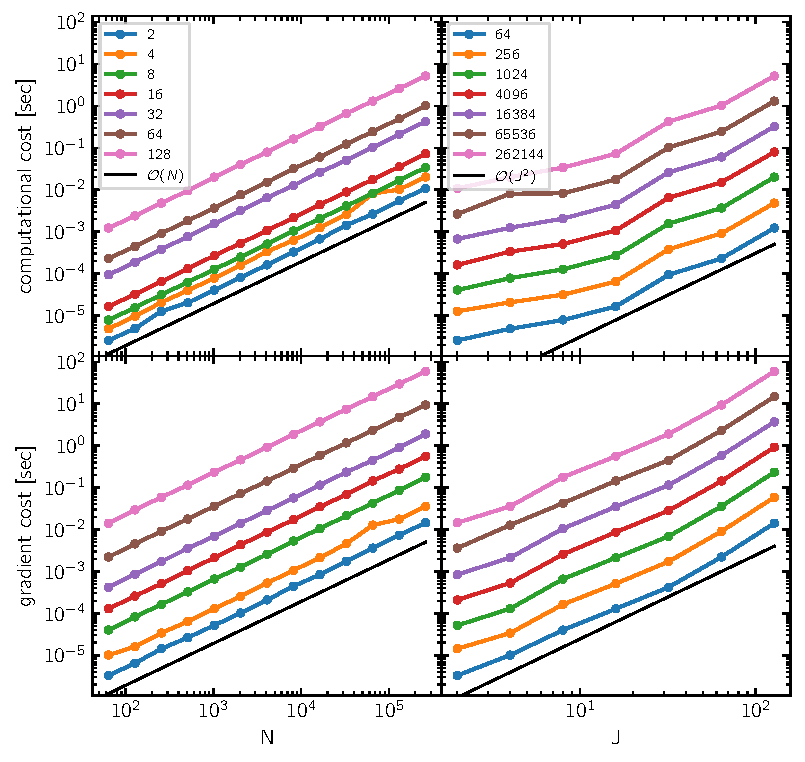
\includegraphics[width=0.9\textwidth]{figure.pdf}
\caption{%
    Scaling.
\figurelabel{figure}}
\end{center}
\end{figure}

%\acknowledgements
%It is a pleasure to thank
%  Patrick Cooper,
%  Boris Leistedt,
%  Bernhard Sch\"olkopf, and
%  Dun Wang
%for helping us understand all of this.

\bibliography{celerite}

\end{document}
